\documentclass[11pt]{article}

\usepackage[utf8]{inputenc}
\usepackage[T1]{fontenc}
\usepackage[margin=2.4cm]{geometry}
\usepackage{tikz}
\usepackage{graphicx}
\usepackage{float}
\usepackage{xcolor}
\usepackage{enumitem}
\usepackage{booktabs}
\usepackage{amssymb}
\usepackage{hyperref}
\usetikzlibrary{arrows.meta, positioning, fit, backgrounds, decorations.pathreplacing}

\hypersetup{colorlinks=true, urlcolor=blue!60!black, linkcolor=black}
\renewcommand{\figurename}{Figura}

\definecolor{boxblue}{HTML}{2C5F8A}
\definecolor{boxgray}{HTML}{4A4A4A}
\definecolor{cellfill}{HTML}{EAF2FB}

\tikzset{
  mod/.style={draw=boxblue, thick, rounded corners, fill=boxblue!8,
              align=center, inner sep=6pt, font=\small},
  big/.style={draw=boxblue, very thick, rounded corners, fill=boxblue!4,
              align=center, inner sep=8pt, font=\small},
  cell/.style={draw=boxgray, thick, minimum width=1.3cm, minimum height=0.9cm,
               fill=cellfill, font=\ttfamily},
  flow/.style={-{Stealth[length=2.5mm]}, thick, draw=boxgray},
  biflow/.style={{Stealth[length=2.5mm]}-{Stealth[length=2.5mm]}, thick, draw=boxgray},
}

\title{\vspace{-1.2cm}\textbf{riscy}: simulador del ISA RISC-V (RV32I)}
\author{Steve Andy Ildefonso Santos \\ \texttt{steve.ildefonso@utec.edu.pe}}
\date{CS3051 -- Arquitectura de Computadores 2026-I \quad\textbar\quad HW\#6, Tarea 4}

\begin{document}
\maketitle
\vspace{-0.6cm}

\noindent\textbf{Repositorio:} \url{https://github.com/stiffis/riscy}

\section{Resumen}

\textbf{riscy} es un simulador del conjunto de instrucciones base de RISC-V
(\textbf{RV32I}, 32 bits) escrito en \textbf{Python} (solo biblioteca estándar).
Carga un programa ya compilado desde un archivo, mantiene el estado
arquitectónico de la CPU --- \texttt{PC}, 32 registros y memoria --- y ejecuta el
código máquina \textbf{paso a paso}, permitiendo inspeccionar registros y memoria
en cualquier punto a través de una interfaz de terminal (TUI).

Es un simulador \emph{funcional} a nivel de ISA: ejecuta una instrucción completa
por paso, que es exactamente la semántica arquitectónica del repertorio.

\section{Arquitectura del programa}

El simulador separa tres responsabilidades: cargar el programa, ejecutarlo y
mostrarlo. El modelo de ejecución se esconde detrás de una interfaz
(\texttt{CPUBackend}), de modo que la TUI no depende de un backend concreto.

\begin{center}
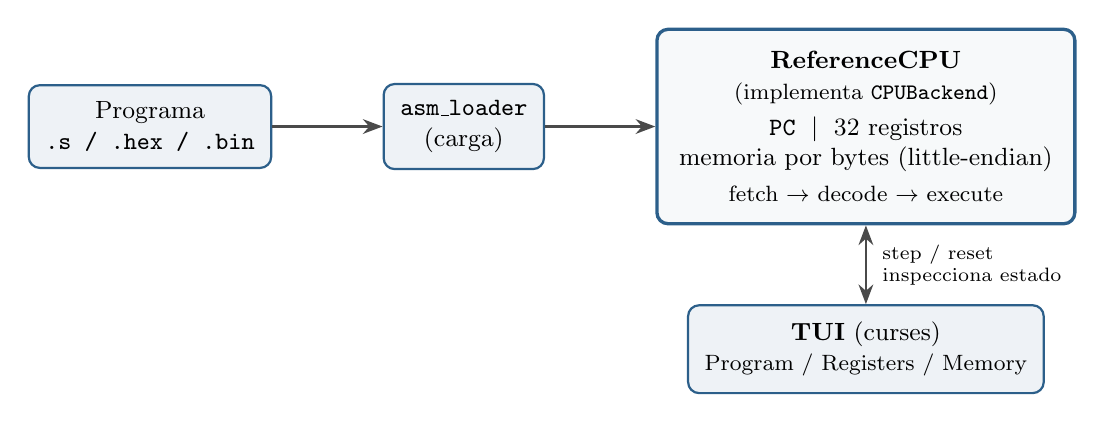
\begin{tikzpicture}[node distance=1.0cm and 1.4cm]
  \node (file)   [mod] {Programa\\\texttt{.s / .hex / .bin}};
  \node (loader) [mod, right=of file] {\texttt{asm\_loader}\\(carga)};
  \node (cpu)    [big, right=of loader] {\textbf{ReferenceCPU}\\\footnotesize(implementa \texttt{CPUBackend})\\[2pt]
                  \texttt{PC} \;\textbar\; 32 registros\\ memoria por bytes (little-endian)\\[2pt]
                  \footnotesize fetch $\rightarrow$ decode $\rightarrow$ execute};
  \node (tui)    [mod, below=1.0cm of cpu] {\textbf{TUI} (curses)\\\footnotesize Program / Registers / Memory};

  \draw[flow] (file) -- (loader);
  \draw[flow] (loader) -- (cpu);
  \draw[biflow] (cpu) -- node[right, font=\scriptsize, align=left]{\;step / reset\\\;inspecciona estado} (tui);
\end{tikzpicture}
\end{center}

\noindent
La interfaz \texttt{CPUBackend} define el contrato (\texttt{pc}, \texttt{registers},
\texttt{memory}, \texttt{step()}, \texttt{reset()}, breakpoints, \texttt{run\_to\_end}, \dots).
\texttt{ReferenceCPU} es la implementación de referencia del ISA. Gracias a esta
separación, el mismo frontend puede manejar otros backends sin cambios.

\subsection*{Ciclo de ejecución}

Cada paso (\texttt{step}) ejecuta una instrucción completa:

\begin{center}
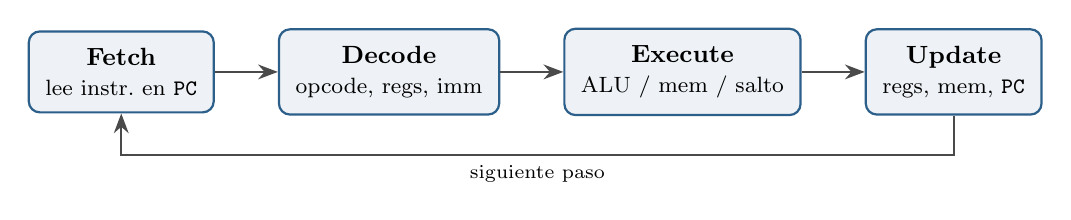
\begin{tikzpicture}[node distance=0.8cm]
  \node (f) [mod] {\textbf{Fetch}\\\footnotesize lee instr.\ en \texttt{PC}};
  \node (d) [mod, right=of f] {\textbf{Decode}\\\footnotesize opcode, regs, imm};
  \node (e) [mod, right=of d] {\textbf{Execute}\\\footnotesize ALU / mem / salto};
  \node (w) [mod, right=of e] {\textbf{Update}\\\footnotesize regs, mem, \texttt{PC}};
  \draw[flow] (f) -- (d);
  \draw[flow] (d) -- (e);
  \draw[flow] (e) -- (w);
  \draw[flow] (w.south) -- ++(0,-0.5) -| node[below, pos=0.25, font=\scriptsize]{siguiente paso} (f.south);
\end{tikzpicture}
\end{center}

\section{Modelo de memoria}

La memoria es \textbf{plana, byte-addressable y little-endian}, con espacio de
direcciones de 32 bits, tal como exige el enunciado. Se implementa de forma
dispersa (solo se materializan las celdas escritas), por lo que cualquiera de los
4\,GiB direccionables es accesible sin reservar memoria real.

Una palabra de 32 bits ocupa 4 celdas consecutivas; el byte menos significativo
va en la dirección más baja (little-endian). Por ejemplo, \texttt{0x12345678} en
la dirección \texttt{0x00}:

\begin{center}
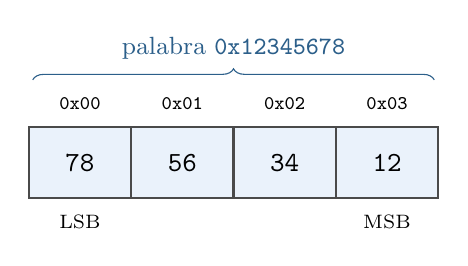
\begin{tikzpicture}
  \foreach \i/\b in {0/78, 1/56, 2/34, 3/12} {
    \node[cell] (c\i) at (\i*1.3, 0) {\b};
    \node[font=\scriptsize\ttfamily] at (\i*1.3, 0.75) {0x0\i};
  }
  \node[font=\scriptsize] at (0,-0.75) {LSB};
  \node[font=\scriptsize] at (3*1.3,-0.75) {MSB};
  \draw[decorate, decoration={brace, amplitude=4pt}, boxblue]
        (-0.6,1.05) -- (3*1.3+0.6,1.05)
        node[midway, above=4pt, font=\small]{palabra \texttt{0x12345678}};
\end{tikzpicture}
\end{center}

\noindent
Esto permite soportar accesos de byte (\texttt{lb}/\texttt{sb}), media palabra
(\texttt{lh}/\texttt{sh}) y palabra (\texttt{lw}/\texttt{sw}), con extensión de
signo o de ceros según corresponda. El puntero de pila (\texttt{sp}) se
inicializa en el \emph{reset} para que el código que usa stack (p.\,ej.\
recursión) corra sin configuración extra.

\section{Conjunto de instrucciones}

Se implementa el repertorio base \textbf{RV32I} completo:

\begin{itemize}[noitemsep, leftmargin=1.4em]
  \item \textbf{Loads/Stores:} \texttt{lb lh lw lbu lhu sb sh sw}
  \item \textbf{ALU (inmediato):} \texttt{addi slti sltiu xori ori andi slli srli srai}
  \item \textbf{ALU (registro):} \texttt{add sub sll slt sltu xor srl sra or and}
  \item \textbf{Upper:} \texttt{lui auipc}
  \item \textbf{Saltos/Branches:} \texttt{beq bne blt bge bltu bgeu jal jalr}
\end{itemize}

\noindent
Las instrucciones no soportadas se reportan explícitamente (la ejecución se
detiene indicando \emph{Illegal instruction}).

\section{Uso}

El programa se carga en la dirección \texttt{0x00000000}. Formatos aceptados:
ensamblador (\texttt{.s}/\texttt{.asm}), hexadecimal (\texttt{.txt}/\texttt{.hex})
y binario crudo (\texttt{.bin}, p.\,ej.\ exportado desde CPUlator).

\begin{verbatim}
    python3 app.py tests/programs/riscvtest.bin
\end{verbatim}

\noindent
Controles principales: \texttt{s} (un paso), \texttt{c} (continuar hasta
breakpoint), \texttt{b} (breakpoint), \texttt{j/k} (scroll), \texttt{r} (reset),
\texttt{?} (ayuda), \texttt{q} (salir).

\begin{figure}[H]
  \centering
  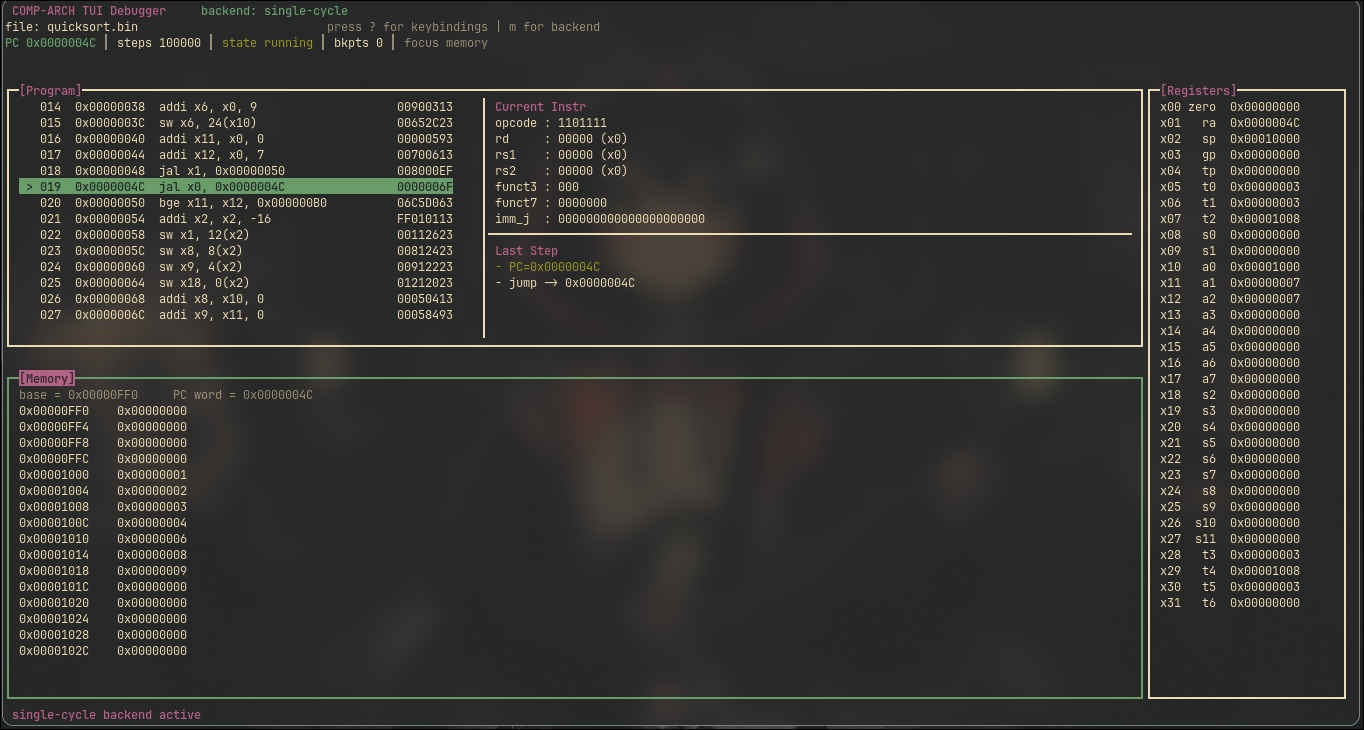
\includegraphics[width=\linewidth]{img/tui.png}
  \caption{Interfaz de terminal: panel de programa con desensamblado, registros y
           memoria. El \texttt{PC} y los valores que cambian se resaltan en cada paso.}
\end{figure}

\section{Validación}

El simulador se valida con pruebas automatizadas (\texttt{unittest}), incluyendo
los tres programas recomendados en el enunciado, \textbf{compilados} con una
toolchain RISC-V a binario crudo:

\begin{center}
\small
\begin{tabular}{@{}lll@{}}
\toprule
\textbf{Programa} & \textbf{Qué hace} & \textbf{Resultado} \\
\midrule
\texttt{riscvtest} & subset add/sub/and/or/slt/lw/sw/beq/jal & \texttt{Mem[100]=25} \checkmark \\
árbol simétrico    & \texttt{is\_symmetric} sobre árbol aplanado & \texttt{a0=1} \checkmark \\
quicksort          & ordena \{6,4,3,2,1,8,9\} en \texttt{0x1000} & \{1,2,3,4,6,8,9\} \checkmark \\
\bottomrule
\end{tabular}
\end{center}

\noindent
Los programas de árbol y quicksort usan recursión y pila, y entre los tres
ejercitan todo el repertorio aritmético/lógico, validando el simulador de
extremo a extremo.

\section{Extras}

Más allá de lo obligatorio, riscy incluye: un \textbf{desensamblador} integrado
(muestra la instrucción original en ejecución), \textbf{breakpoints} y
ejecución controlada (\emph{continue}, \emph{run-to-cursor}), una TUI con paneles
de programa, registros y memoria, y una arquitectura de \textbf{backends
intercambiables} que permite, de forma experimental, manejar también un pipeline
RISC-V en Verilog mediante Verilator.

\end{document}
